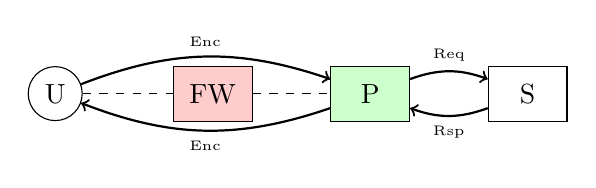
\begin{tikzpicture}[
    scale=0.4,
    node distance=2cm,
    user/.style={circle,draw,minimum size=0.6cm},
    proxy/.style={rectangle,draw,fill=green!20,minimum width=1cm,minimum height=0.7cm},
    server/.style={rectangle,draw,minimum width=1cm,minimum height=0.7cm},
    firewall/.style={rectangle,draw,fill=red!20,minimum width=1cm,minimum height=0.7cm}
]
    % Define nodes
    \node[user] (user) {U};
    \node[firewall] (fw) [right of=user] {FW};
    \node[proxy] (proxy) [right of=fw] {P};
    \node[server] (server) [right of=proxy] {S};

    % Draw arrows and connections
    \draw[->,thick] (user) to[bend left=20] node[above,font=\tiny] {Enc} (proxy);
    \draw[dashed] (user) -- (fw);
    \draw[dashed] (fw) -- (proxy);
    \draw[->,thick] (proxy) to[bend left=20] node[above,font=\tiny] {Req} (server);
    \draw[->,thick] (server) to[bend left=20] node[below,font=\tiny] {Rsp} (proxy);
    \draw[->,thick] (proxy) to[bend left=20] node[below,font=\tiny] {Enc} (user);
\end{tikzpicture}